\documentclass{beamer}

\usepackage{graphicx}
\usepackage{minted}
\usetheme{Frankfurt}

\title{Introduction to python}
\author{Jadavpur University Code Club}
\titlegraphic{
\includegraphics[width=.5\textwidth]{./img/python_o_1269231.jpg}}
\date{}

\begin{document}

\maketitle

\begin{frame}[fragile]{The hello world program}
	\begin{minted}{python}
		print("hello world")
	\end{minted}
	\pause
	\begin{center}
		
\includegraphics[width=.3\textwidth]{./img/images.jpg}
	\end{center}
\end{frame}

\begin{frame}
	\begin{center}
		
\includegraphics[width=0.7\textwidth]{./img/main-qimg-e7eaa6e92e42b3df3a851a961fdf7540.jpg}
	\end{center}
\end{frame}

\begin{frame}[fragile]{Running the code}
	\Large{Two ways to do it:}
	\begin{itemize}
		\item Interactive mode
		\item Shell mode
	\end{itemize}
\end{frame}

\begin{frame}[fragile]{Variables}
	\begin{minted}{python}
		x = 1.0
		y = "hello world"
	\end{minted}
	\begin{center}
		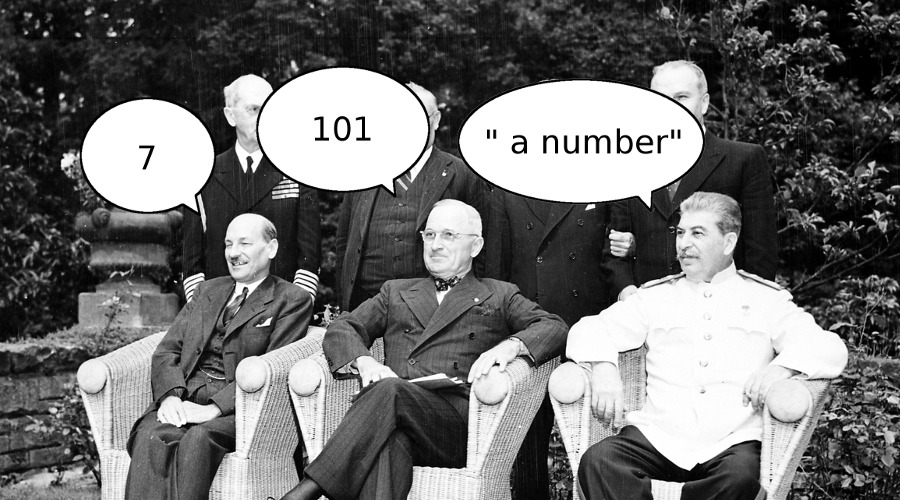
\includegraphics[width=.7\textwidth]{./img/variables.jpg}
	\end{center}
\end{frame}

\begin{frame}{Variable naming conventions and rules}
	You must assign a value to a variable before you can use it, 
	even if that value is zero or empty.
	\\
	\\
	{\Large Rules:}
	\begin{itemize}
		\item Variable names must start with a letter or an underscore (\_)
		\item The remainder of your variable name may consist of letters
			numbers and underscores
		\item The names are case sensitive
	\end{itemize}
\end{frame}

\begin{frame}{Data types}
	\begin{itemize}
		\item int
		\item float
		\item list
		\item tuple
		\item strings
	\end{itemize}
\end{frame}

\begin{frame}[fragile]{If Else}
	\begin{minted}{python}
		if x<0:
	 	  print("Negative")
		elif x==0:
		  print("Zero")
		else:
		  print("Positive")
	\end{minted}
\end{frame}

\begin{frame}[fragile]{Indentation is important}
\begin{minted}{python}
	if foo:
	    if bar:
	        print(x)
	else:
	    print(y)
\end{minted}
\end{frame}

\begin{frame}
	\begin{center}
		
\includegraphics[width=0.6\textwidth]{./img/neo.jpg}
	\end{center}
\end{frame}

\end{document}
